\chapter{Upgrade on the ATLAS Calorimeter Trigger}
After the LHC operation with $\sqrt{s}=13$ from 2015 to 2018, it is now in the long-shutdown period (LS2) to prepare for the Run~3 operation which will start in 2021. The major upgrades in this period are to enhance the LHC energy for proton-proton collision as well the luminosity. Meanwhile, three main upgrades will be also performed on the ATLAS detector: the new small wheel (NSW) in the muon spectrometer\cite{STELZER20161160}, the fast tracking trigger at HLT\cite{Shochet:1552953}, and the new L1Calo infrastructure. One of the main purposes of the two upgrades is to improve the trigger rate for better recognition on the physical objects. This chapter will be dedicated to the L1Calo Run~3 upgrade from the hardware design, preparation of the software, to expected performance of the new L1Calo infrastructure.   
\section{LHC Run~3 Upgrade}
After the operation of Run~2 (2015-2018), the LHC is now undergoing the Long Shutdown period (LS2) during which a couple of upgrades and maintenance will be taken to enhance the LHC performance to prepare for the upcoming operation in 2021. This is to bring the LHC to the design energy of $7~TeV$ for each beam and also enhance the instantaneous luminosity to $2\times10^{34}~cm^{-2}s^{-1}$ with estimated $\sim 70$ pile-ups per bunch crossing which doubles the nominal LHC luminosity. This operation is expected to last for three years delivering the integrated data of $300~fb^{-1}$ by the end of this period. This upgrade plan could also be taken as the preceding work for the High-Luminosity LHC (HL-LHC) which will keep the beams at $7~TeV$, but the instantaneous luminosity will increase to $7.5\times10^{34}~cm^{-2}s^{-1}$ for which the pile-ups will go up to 200 per bunch crossing. The LHC upgrade road map and the estimated instantaneous luminosity could be seen in Fig.~\ref{Fig:LHC_upgrade}.
\begin{figure}[!h]                
	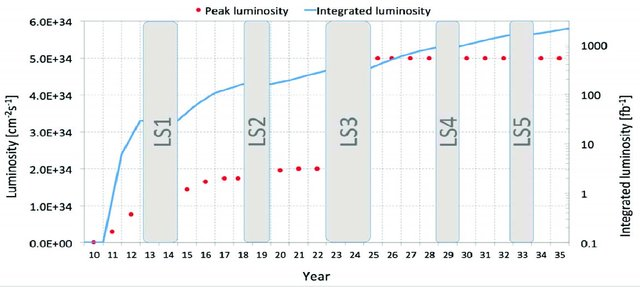
\includegraphics[width=0.9\textwidth]{Chapter6/The-LHC-upgrade-schedule-and-associated-luminosity.jpg}
	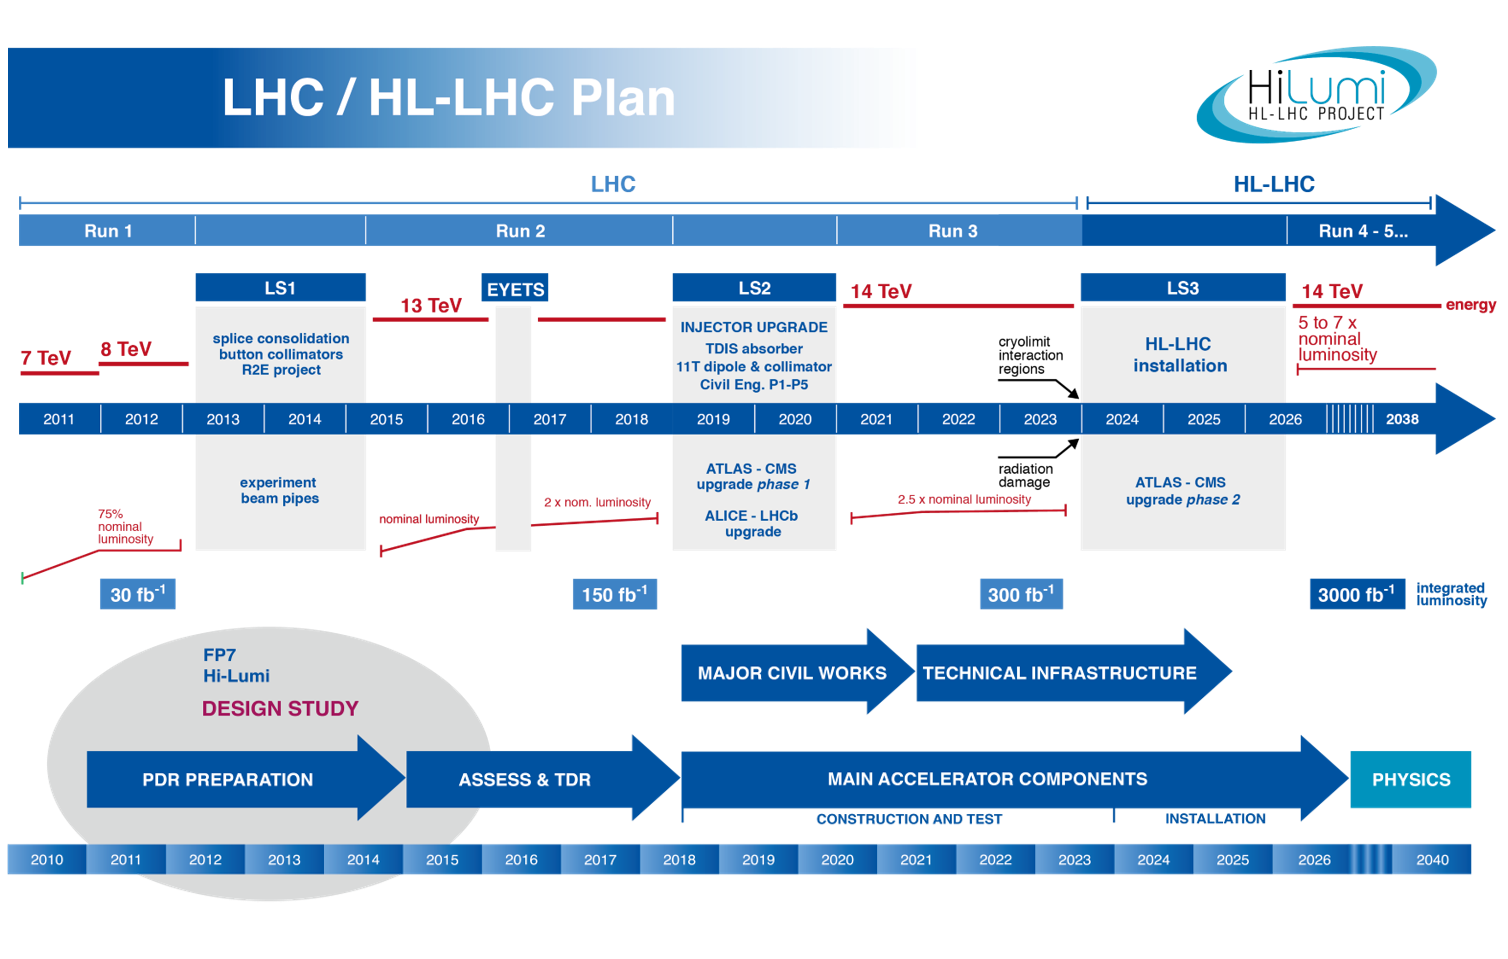
\includegraphics[width=0.9\textwidth]{Chapter6/Schedule_HL.png}
	\begin{center}
		\caption{The LHC upgrade plan (top)\cite{schedule} and the instantaneous luminosity (bottom)\cite{Atlas:2019qfx} for the upcoming 10 years with the estimated integrated data.}
		\label{Fig:LHC_upgrade}            
	\end{center}
\end{figure} 
\noindent
\\
\\The major upgrade of this project is that the injector of beams will be replaced by the new LINAC4, and the LINAC2 will just retire from 40~years of operation. The major difference between the LINAC2 and LINAC4 is that the LINAC4 will accelerate negatively charged hydrogen ions ($H^{-1}$), and the electrons will be stripped off in the PSB, which design is intended to concentrate the beams with better stability\cite{LINAC4}. Furthermore, the CERN acceleration complex (Fig.~\ref{Mobs:2197559}) will also upgrade the RF cavities for the energy upgrade. For the LHC itself, the upgrade will take place in the magnet systems for which more than 20 magnets will be replaced, and the new superconductor technology will also be employed with the new magnet material which can afford the even higher magnetic field of $\sim 10~Tesla$ (the original material can only take the magnetic field up to $\sim 9~Tesla$). 
\\
\\This upgrade project is aiming to refine the present physics results. Firstly, the Higgs boson properties like the couplings to other particles or themselves could be measured with better precision to verify the SM predictions. Secondly, most of the SM interactions have the cross-sections as a function of the collision centre-of-mass energy, and the new operation energy could provide another measurement points. Thirdly, the increase of collected data will benefit the new physics search giving a better separation on the test statistics between hypotheses, and this will enhance the sensitivity to the hidden particles. \cite{Atlas:2019qfx} has summarized all the studies for expected results with the Run~3 LHC data.
\section{Hardware Design of the Run~3 ATLAS Calorimeter Trigger}
To incorporate the upcoming LHC upgrades, the ATLAS hardware calorimeter trigger system is scheduled to undergo a series of upgrade to cope with the unprecedented luminosity. The full scheme could be seen in Fig.~\ref{Fig:l1calo_scheme}.
\begin{figure}[!h]                
	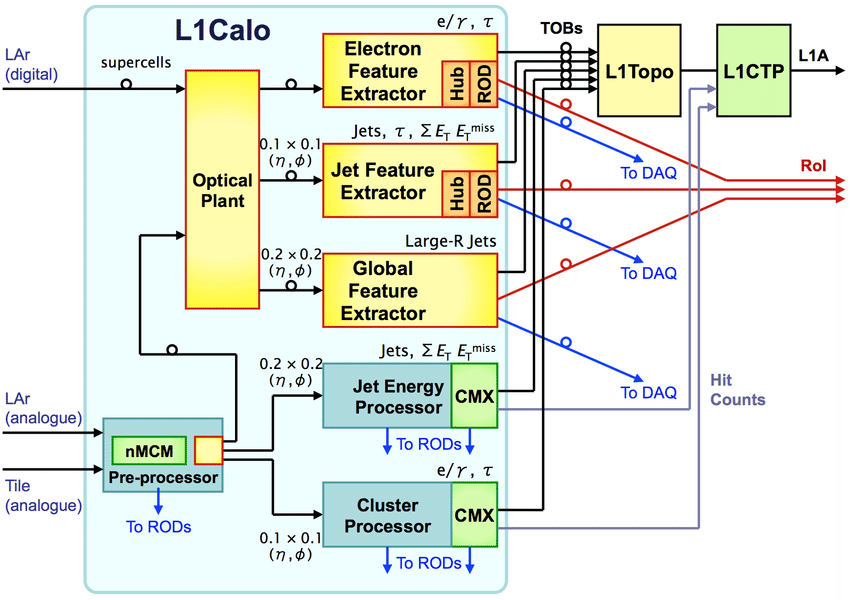
\includegraphics[width=0.9\textwidth]{Chapter6/L1Calo.png}
	\begin{center}
		\caption{The L1Calo hardware scheme in the Run~3 operation\cite{Schwienhorst:2016efd}}
		\label{Fig:l1calo_scheme}            
	\end{center}
\end{figure}
\noindent
For the Run~2 scheme, the L1Calo trigger has the analogue inputs from both the tile and LAr detectors. However, for the Run~3 operation, the LAr output will be digitized, and the tile will remain the same. In this case, the new Run~3 system will be running in parallel with the Run~2 one to have 